
\section{General counter}


\begin{figure}[H]
    \centering
    \begin{subfigure}[t]{0.2\textwidth}
        \centering
        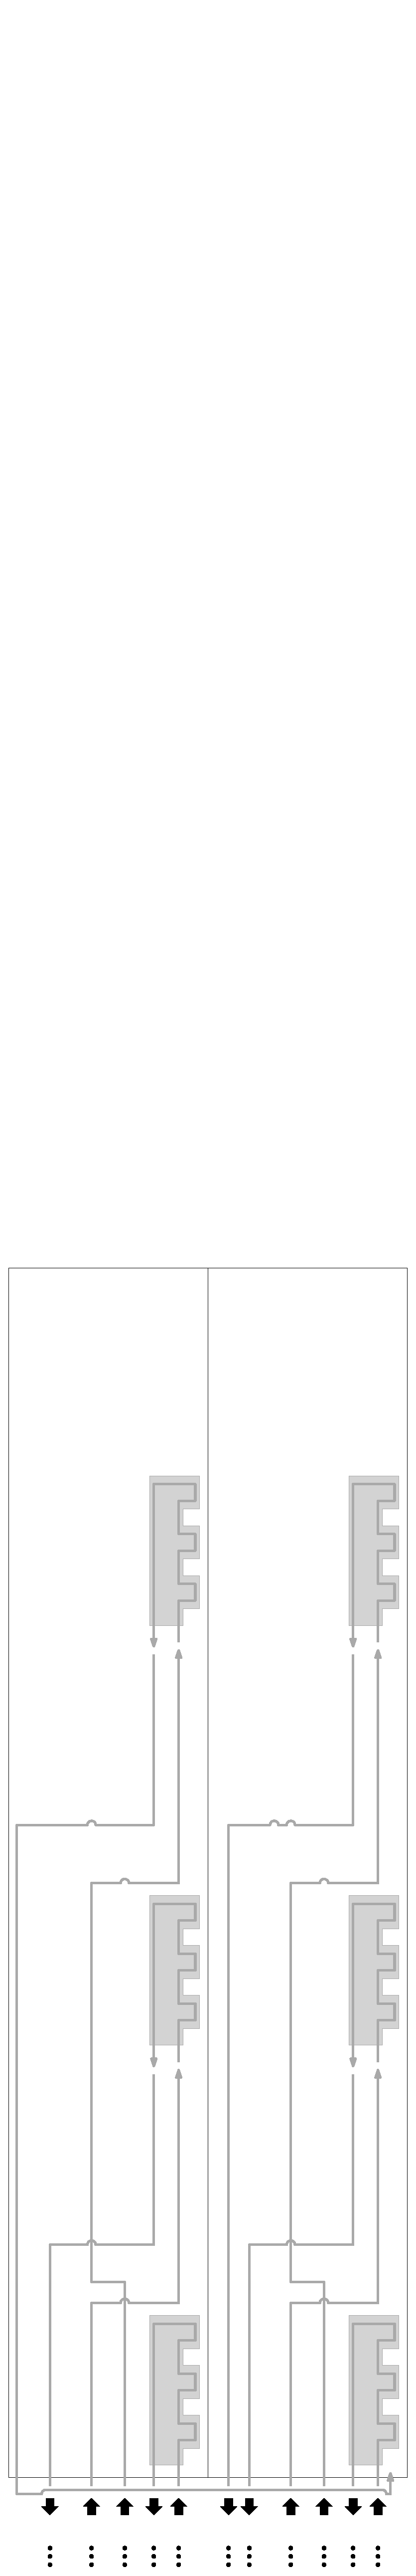
\includegraphics[width=0.6in]{counter_read_start_general_case3_middle_level}
        \caption{\label{fig:counter_read_start_general_case3_middle_level} A ``clean'' counter row, before any reading has started.}
    \end{subfigure}%
    ~
    \begin{subfigure}[t]{0.2\textwidth}
        \centering
        \includegraphics[width=0.6in]{counter_read_digit1_return_read_digit2_general_case3_middle_level}
        \caption{\label{fig:counter_read_digit1_return_read_digit2_general_case3_middle_level} Read digit 1 in the current row, write digit 1 in the next row.}
    \end{subfigure}%
    ~
    \begin{subfigure}[t]{0.2\textwidth}
        \centering
        \includegraphics[width=0.6in]{counter_read_digit2_return_read_digit3_general_case3_middle_level}
        \caption{\label{fig:counter_read_digit2_return_read_digit3_general_case3_middle_level} Read digit 2 in the current row, write digit 2 in the next row.}
    \end{subfigure}%
    ~
    \begin{subfigure}[t]{0.2\textwidth}
        \centering
        \includegraphics[width=0.6in]{counter_read_digit3_return_read_digit1_general_case3_middle_level}
        \caption{\label{fig:counter_read_digit3_return_read_digit1_general_case3_middle_level} Read digit 3 in the current row, write digit 3 in the next row.}
    \end{subfigure}%

    \caption{\label{fig:counter_read_digit_return_read_digit_general_case3}
    This illustrates how a counter reads and writes a digit region, in a general sense.
    The counter starts in the rightmost digit region by reading the bottommost digit within
    that region. After reading digit 1 in the current row, the corresponding digit region in
    the next row be started in the next row. The counter writes the first digit in the next 
    row, and then returns to the second digit in the current digit region.
    Once all the digits in the current digit region are read and written into the next row,
    the counter can then do one of the following: continue reading digits by moving on to the 
    next digit region, cross back all the way to the right of the rectangle and start reading 
    the next row, or halt.}
\end{figure}

